\section{The viscous Burgers equation}

We will illustrate the application of DPG to nonlinear problems using a viscous Burgers' equation on domain $\Omega = [0,1]^2 \in \mathbb{R}^2$
\[
\pd{\left(u^2/2\right)}{x} + \pd{u}{y} - \epsilon \Delta u = f.
\]
If we remove the viscous term, the above problem reduces to the form of the 1D transient Burgers equation, whose solution we can determine via the method of characteristics.  For boundary conditions 
\[
u(x,y) = 1-2x, \quad x = 0, y = 0,
\]
the solution forms a shock discontinuity starting at $(x,y) = (.5,.5)$, which then propagates upward in the $y$-direction.  The addition of the viscous term smears this discontinuity, leading to a solution with a smooth shock of width $\epsilon$.  

We begin by writing the equation as a first order system.  Defining $\beta(u) = \LRp{u/2,1}$, the above Burgers equation can be written as 
\begin{align*}
\div\left(\beta(u)u-\sigma\right) &=f \\
\frac{1}{\epsilon}\sigma - \grad u &=0.
\end{align*}
Analogously to the convection-diffusion problem, the DPG nonlinear variational formulation can then be given
\[
b\left(\left(u,\sigma,\widehat{u},\widehat{f}_n\right),\left(v,\tau\right)\right) = \LRp{u,\div \tau - \beta(u) \cdot \grad v} + \LRp{\sigma, \frac{1}{\epsilon}\tau + \grad v} + \LRa{\widehat{u},\tau\cdot n} + \LRa{\widehat{f}_n,v} = \LRp{f,v}
\]
Linearizing the above then gives us 
\begin{align*}
b_u\left(\left(\Delta u,\sigma,\widehat{u},\widehat{f}_n\right),\left(v,\tau\right)\right) &= \LRp{\Delta u,\div \tau - \vecttwo{u}{1} \cdot \grad v} + \LRp{\sigma, \frac{1}{\epsilon}\tau + \grad v} + \LRa{\widehat{u},\tau\cdot n} + \LRa{\widehat{f}_n,v} \\
&= \LRp{u,\div \tau - \beta(u)\cdot \grad v} 
\end{align*}
Notice that the nonlinear term is only dependent on $u$, and thus there is no need to linearize in the variables $\sigma$, $\widehat{u}$, and $\widehat{f}_n$.  

Since the linearized Burgers' equation is of the form of a convection-diffusion problem with non-homogeneous load, we adopt the test norm described in Section~\secref{sec:testNormSec} with convection vector $\beta = (u,1)$.  

Recall that we did not linearize in the flux variables $\widehat{u}$ and $\widehat{f}_n$, so we can directly apply the nonlinear boundary conditions to our variational formulation.  Additionally, since Burgers' equation does not have any physical constraints, we can employ a direct Newton iteration to solve the nonlinear equation.  The adaptivity algorithm is identical to the greedy algorithm described previously, except that the linear solve is replaced by a nonlinear solve.  The results of an adaptive simulation are shown in Figure~\ref{fig:BurgersShock} for $\epsilon = 1e-4$.  

\begin{figure}[!h]
\centering
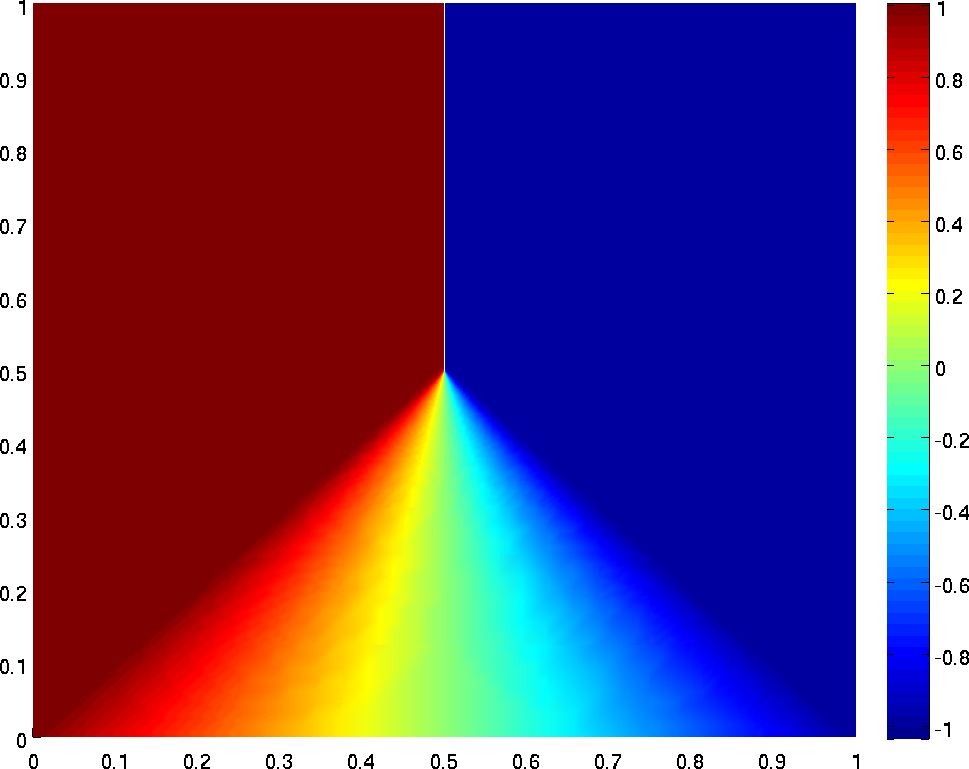
\includegraphics[scale=.45]{figs/burgers1e4.png}
\caption{Shock solution for Burgers' equation with $\epsilon = 10^{-4}$.} 
\label{fig:BurgersShock}
\end{figure}

